%%% LaTeX Template: Two column article
%%%
%%% Source: http://www.howtotex.com/
%%% Feel free to distribute this template, but please keep to referal to http://www.howtotex.com/ here.
%%% Date: February 2011

%%% Preamble
\documentclass[	DIV=calc,%
							paper=a4,%
							fontsize=9.8pt,%
							twocolumn]{scrartcl}	 					% KOMA-article class

\usepackage{lipsum}													% Package to create dummy text
\usepackage{float}
\usepackage[english]{babel}										% English language/hyphenation
\usepackage[protrusion=true,expansion=true]{microtype}				% Better typography
\usepackage{amsmath,amsfonts,amsthm}					% Math packages
\usepackage[pdftex]{graphicx}									% Enable pdflatex
\usepackage[svgnames]{xcolor}									% Enabling colors by their 'svgnames'
\usepackage[hang, small,labelfont=bf,up,textfont=it,up]{caption}	% Custom captions under/above floats
\usepackage{epstopdf}												% Converts .eps to .pdf
\usepackage{subfig}													% Subfigures
\usepackage{booktabs}												% Nicer tables
\usepackage{fix-cm}													% Custom fontsizes



%%% Custom sectioning (sectsty package)
\usepackage{sectsty}													% Custom sectioning (see below)
\allsectionsfont{%															% Change font of al section commands
	\usefont{OT1}{phv}{b}{n}%										% bch-b-n: CharterBT-Bold font
	}

\sectionfont{%																% Change font of \section command
	\usefont{OT1}{phv}{b}{n}%										% bch-b-n: CharterBT-Bold font
	}



%%% Headers and footers
\usepackage{fancyhdr}												% Needed to define custom headers/footers
	\pagestyle{fancy}														% Enabling the custom headers/footers
\usepackage{lastpage}	

% Header (empty)
\lhead{}
\chead{}
\rhead{}
% Footer (you may change this to your own needs)

\cfoot{}
\rfoot{\footnotesize page \thepage\ of \pageref{LastPage}}	% "Page 1 of 2"
\renewcommand{\headrulewidth}{0.0pt}
\renewcommand{\footrulewidth}{0.4pt}



%%% Creating an initial of the very first character of the content
\usepackage{lettrine}
\newcommand{\initial}[1]{%
     \lettrine[lines=3,lhang=0.3,nindent=0em]{
     				\color{black}
     				{\textsf{#1}}}{}}



%%% Title, author and date metadata
\usepackage{titling}															% For custom titles

\newcommand{\HorRule}{\color{black}%			% Creating a horizontal rule
									  	\rule{\linewidth}{1pt}%
										}

\pretitle{\vspace{-30pt} \begin{flushleft} \HorRule 
				\fontsize{24}{24} \usefont{OT1}{phv}{b}{n} \color{black} \selectfont 
				}
\title{Design, Implementation and Evaluation of a Robust Speech Recognition System}					% Title of your article goes here
\posttitle{\par\end{flushleft}\vskip 0.5em}

\preauthor{\begin{flushleft}
					\large \lineskip 0.5em \usefont{OT1}{phv}{b}{sl} \color{black}}
\author{Luke M. Garrigan 800086495 |   Shane J. Sturgeon 100082588
 }											% Author name goes here
\postauthor{\footnotesize \usefont{OT1}{phv}{}{sl} \color{Black} 
												% Institution of author
					\par\end{flushleft}\HorRule}

\date{}																				% No date



%%% Begin document
\begin{document}
\maketitle

\thispagestyle{fancy} 			% Enabling the custom headers/footers for the first page 
% The first character should be within \initial{}

\section*{Abstract}
In this paper we investigate various parameters and techniques to build a robust speech recogniser. We experiment with numerous approaches to speech collection, feature extraction, acoustic modelling and noise compensation. More specifically, adjusting methods for recording the data with a multitude of equipment, name ordering and sample rate. We test the performances of  Linear frequency cepstral coefficients (LFCC) and Mel-frequency cepstral coefficients (MFCC) under a number of scenarios, and find that although not as widely used as MFCC, LFCC  is as robust as when babble noise is added. We add noise and babble to our model and test different methods of noise compensation such as spectral subtraction and Wiener Filter. We also add noise to our training data to test the speech models on noisy speech. The software was modelled around 22 names: Daniel, Peyton, Peter, Owen, Dan, Justinas, Luke, Samuel, Brandon, Meron, Louise, Wazzy, Edward, James, Michael, Shane, Jamie, Berk, Marcio, Will, Oliver, Sam. 

\section{Introduction}
The aim of this work is to examine the best techniques available for an accurate speech recognition system with the use of a combination of programs. MATLAB is used  for implementing feature extraction and noise compensation. SFS (Speech Filing System) is used for annotating the audio and HTK (Hidden Markov Model Toolkit) for the development of the speech recogniser by building and manipulating hidden Markov models

\section{Speech Collection}
When recording data to train the speech recognition model, we recorded each name 20 times in a row. The speech was captured in a quiet room with a sensitive microphone to pick up on the clarity of speech and eliminate the majority of noise. It was decided that the recorded speech should be as clean as possible so that noise could be added to the recordings for alternate tests  at a later date.

The sampling rate of the speech was recorded at  44Khz allowing for down sampling to the requirements specification of certain experiments. After all training data had been collected we then recorded all the testing speech, this consisted of all 22 names spoken consecutively. In particular, we recorded the testing data in no explicit order; so the 22 names were scrambled and then spoken. This process was completed 20 times. We recorded the testing data in this manner in the hope of grasping a more detailed representation of how accurate the training model is.

Once the training model had been tested, we further implemented additional training data  into the model in the hope of improving the recognition of the system. We did this by recording each name a further 10 times and tested the results against a set test model, then recorded a further 10 names and documented the results. See 6. For further details


\subsection{Annotation Methodology}
After all data had been recorded it had to be labeled to inform HTK of when individual names were being spoken for training and creating confusion matrices. Annotation of the speech utterances were completed with the program SFS, this allowed us to label the beginning and end of each name. The beginning of all the .wav files were annotated with sil which represents silence followed by the next name and sil again once the name utterance had ended.

In figure 1 the green annotation line represents the beginning of the name utterance Edward and the blue line represents the end of the name utterance and the beginning of the silence.

\begin{figure}[ht]
	\centering
	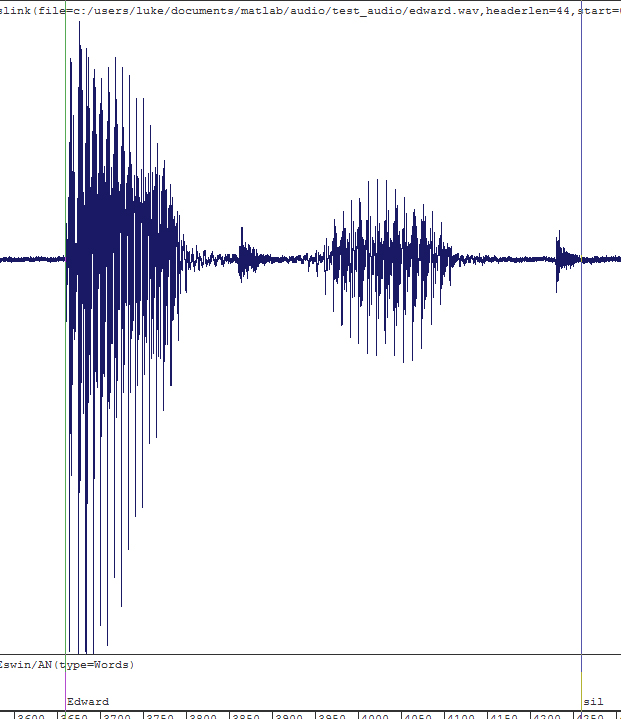
\includegraphics[width=0.3\textwidth]{labelling}
	\captionsetup{justification=centering}
	\caption{SFS labelling example}
\end{figure}

Once the annotations had been made they were exported to a .lab (file extension needed for HTK) file which contains where in the utterance the speech starts in nanoseconds followed by the word (see table 1). 
\begin{table}[h]
	\caption{Labelling of Edward}
	\centering
	\begin{tabular}{llr}
	
		\cmidrule(r){1-3}
		From & To & Name \\
		\midrule
		0 & 8731400 & sil \\
		8731400  & 15092900  & Edward \\
		15092900   & 22764100  & sil \\
	
	\end{tabular}
\end{table}


\section{MFCC Extraction}
HTK cannot create acoustic models from the recorded .wav files as they contain far too much data. Before the acoustic models can be produced we had to pass the speech through our feature extraction algorithm in Matlab to obtain the .MFC vectors used by HTK.

As the data was recorded at 44Khz the first stage of the algorithm was to resample the audio to a lower sample rate, since human speech has a relatively low bandwidth mostly between 100Hz and 8KHz a sampling frequency of 16KHz is sufficient.  

Our feature vector algorithm consists of 8 stages, these are: Pre-Emphasis, Windowing, FFT, Magnitude Spectrum, Filter Bank, Logarithm, DCT and writing to MFC file. 

The .wav file is read into a variable, a hamming window function is applied to the entire speech wave, then the Discrete Fourier Transform Vector is calculated using the FFT() function (Fast Fourier Transform). The DFT vector is then used by the abs() function to get the Magnitude Spectrum, iterating frame by frame over the 
magnitude vector and applying a Filter Bank. Logarithm is applied to the resulting vector and is then used to calculate the Discrete Cosine Transform vector. MFCC headers are added and the DCT vector is written to file. Details of each stage below. 


\subsection{Pre-emphasis}
The first step post resampling was Pre-emphasis, which is designed to increase the magnitude of higher frequencies with respect to the magnitude of lower frequencies this is because the energy content of low frequency sounds is higher than energy of higher frequency sounds. Pre-emphasis was used to spectrally flatten the speech spectrum across frequencies, this was implemented using a high-pass filter, see figure 2.

\begin{figure}[ht]
	\centering
	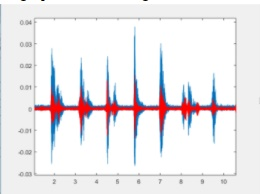
\includegraphics[width=0.4\textwidth]{preemphasis}
	\captionsetup{justification=centering}
	\caption{Pre-emphasis}
\end{figure}

\subsection{Windowing}
Speech is a non-stationary time variant signal, a signal is said to be stationary if its frequency or spectral components do not change over time, it is assumed that human speech is built from a dictionary of phonemes.

\cite{DBLP:journals/taslp/NorholmJC16}
For most phonemes in  language the properties of speech remain constant for a short period of time, roughly (5-100ms). Thus we assume the signal behaves stationary for those time frames. Window functions are used in signal processing to minimise the effect of spectral leakages.
Windowing consists of multiplying the speech signal by a fixed length window with an amplitude that varies smoothly and gradually toward zero at the edges. This makes the endpoints of the waveform touch which results in a continuous waveform. 

We experimented with three different windows: Hamming window, Hanning window and The Blackman-Harris window, all with their unique characteristics. Each window is defined by three attributes:  the offset between successive windows, the shape of the window and how wide the window is (in milliseconds). The speech that is extracted from each window is called a frame. \cite{DBLP:conf/icira/SulistijonoUD16}
\begin{figure}[ht]
	\centering
	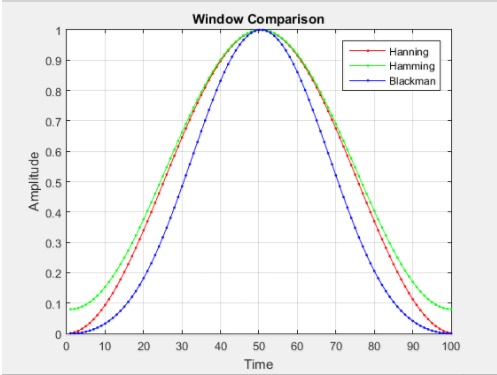
\includegraphics[width=0.4\textwidth]{window}
	\captionsetup{justification=centering}
	\caption{Hamming, Hanning and Blackman-Harris}
\end{figure}



\subsubsection{Hamming Window}
The Hamming window stops just shy of zero at either end (starts at 0.08 and rises to 1 then back to 0.08), meaning that the signal will still have a slight discontinuity.
Both Hamming and Hanning have wide peaks with low sidelobes.
\textit{All graphs were plotted using the same speech utterance}
\begin{figure}[ht]
	\centering
	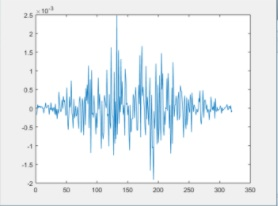
\includegraphics[width=0.4\textwidth]{hamming}
	\captionsetup{justification=centering}
	\caption{Applied hamming window}
\end{figure}


We initially used the Hamming window with a frame size 320 samples (16000 Hz x 0.02s = 320), with an overlap of 50 percent, see figure 4.
 The formula for this window:
\[w(n) = 0.54 - 0.46 \cos \tfrac{2\pi n}{N}\]


\subsubsection{Hanning Window}
Hanning window touches zero at both ends, removing any discontinuity.
 The formula for this window:
\[w(n) = 0.5 - 0.5 \cos \tfrac{2\pi n}{N}\]
\begin{figure}[ht]
	\centering
	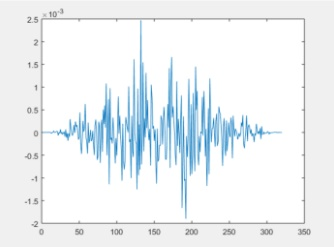
\includegraphics[width=0.4\textwidth]{hanning}
	\captionsetup{justification=centering}
	\caption{Applied hanning window}
\end{figure}

\subsubsection{The Blackman-Harris Window}
The Blackman-Harris window is similar to the Hanning window as it also starts and ends at 0  removing any discontinuity.
The formula for this window: 
\[w(n) = 0.42 - 0.5 \cos (\frac{2\pi n}{M})+0.08\cos (\frac{4\pi n}{M})\]


\begin{figure}[ht]
	\centering
	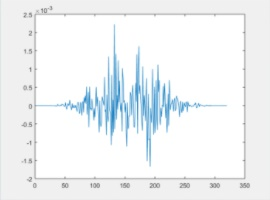
\includegraphics[width=0.4\textwidth]{blackman}
	\captionsetup{justification=centering}
	\caption{Applied Blackman=harris window}
\end{figure}
\subsection{Discrete Fourier Transform (DFT)}
Extracts spectral information to learn how much energy the signal contains at particular frequency bands.
The input to the DFT takes a sampled time-domain signal (our windowed signal), x(n) and returns a sampled frequency-domain signal. \[|X(k)|\]Each frequency-domain point is associated with a particular frequency, and its amplitude shows the energy in the signal at that frequency.

The algorithm for calculating the DFT that we used is Fast Fourier Transform (FFT). FFT rapidly computes the transformation by factorising the DFT matrix into  a product of sparse factors, thus reducing the complexity of the DFT algorithm from O(n2) to O(nlogn).   

Matlab has a built in Fast Fourier Transform function fft(), this was used for our implementation. 

\subsection{Magnitude Spectrum}
The DFT matrix created is passed into the abs() function which calculates the complex magnitude for all the values within the matrix.

The magnitude spectrum value for each bin is established by initially summing the squares of both the real and imaginary components. The square root of this is then found and then the result is divided by the number of bins.

The magnitude spectrum was truncated as there is no need for the reflected half as shown by figure 7.
\begin{figure}[ht]
	\centering
	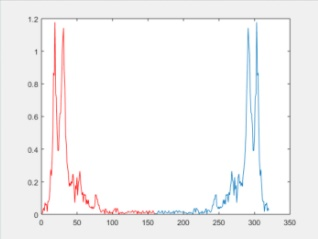
\includegraphics[width=0.4\textwidth]{mag}
	\captionsetup{justification=centering}
	\caption{Reflection in magnitude spectrum}
\end{figure}

\subsection{Filter Banks}
Filter banks are arrangements of lowpass, bandpass highpass filters used for spectral decomposition and composition signals. They provide simple extraction of spectral components of a signal.
 
A low-pass filter removes all spectral components of an input signal that have frequencies higher than some cutoff frequency. A high-pass filter removes spectral components which are lower than a given cutoff frequency. A band-pass filter removes spectral components that occur at frequencies outside of a given range: it only lets through components within a band of frequencies.

\subsubsection{Linear Frequency Cepstral Coefficients}
Mel-frequency cepstral coefficients have been dominantly used in most speech recognition software however it has some limitations. Some speaker characteristics that are associated with the length of the vocal tract are reflected more in higher frequencies in terms of speech. This implication allows us to form a conclusion that a linear scale in frequency may provide some preference over mel scale.

The truncated magnitude is iterated and a mean is taken of every N values (N=fW/P)*, P times. To create a matrix of P averages x number of frames, once iterations has been completed.

After running multiple tests on the number of channels, we found that 20 gave the best results.
*fW = Frame Width, P = Number of Channels
\subsubsection{Mel Frequency Cepstral Coefficients}
Mel-frequency cepstral coefficients (MFCCs) have been widely used as features for speaker recognition, primarily because they’ve been empirically determined to work well for speaker recognition after being developed for speech recognition. \cite{DBLP:conf/interspeech/LeiL09}

The coefficients are calculated on a mel-frequency spacing of filterbank energies, the frequency bands are equally spaced on the mel scale which ensures close approximation to the human auditory system.

\begin{figure}[ht]
	\centering
	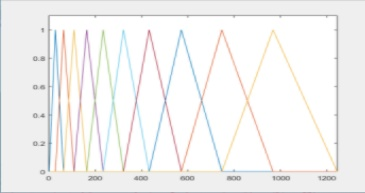
\includegraphics[width=0.5\textwidth]{mel}
	\captionsetup{justification=centering}
	\caption{Mel-scale frequency bands}
\end{figure}

\subsection{Taking The Logarithm}
The log function compresses the dynamic range of the values, as human hearing is more sensitive to slight changes at lower amplitudes rather than higher amplitudes. See figure 8 for example of logarithm function. 

The matrix created from the previous step is passed through the log() function which calculates the log for every value.
\begin{figure}[ht]
	\centering
	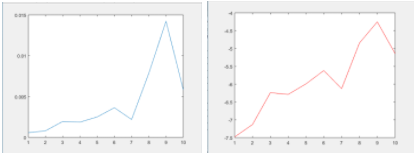
\includegraphics[width=0.5\textwidth]{log}
	\captionsetup{justification=centering}
	\caption{Logarithm applied to first ten filters}
\end{figure}

\subsection{Discrete Cosine Transformation}
In speech recognition, generally a DFT is applied twice in the feature extraction process, initially done post windowing then after the Mel binning. However it is common for speech recognisers to use a Discrete Cosine Transform (DCT) for the second calculation.

The DCT performs a very similar function to DFT: They both decompose a finite-length discrete-time vector into a sum of scaled-and-shifted basis functions. DCT uses only real numbers, while DFT can use complex numbers.

The most common use of DCT is data compression applications. DCT offers a high level of spectral compaction which makes it exceptional at data 
compression. DCT discards the high frequency coefficients to retain only the vocal tract information.


We implemented the DCT using Matlab's built in function dct(). The value from the previous log() was placed into the function for our new vector. \cite{JasonR}

\section{Design and justification of acoustic modelling}
To create and test the acoustic models, the created MFCC vectors were passed through the HTK toolkit using a bash script to automate the entire process

\subsection{HTK}
HTK contains an array of tools for speech analysis, Hidden Markov Model (HMM) training, testing and results analysis. The main features of the HTK library that we use for our analysis are HInnit, HRest, HVite and HResults.

\subsubsection{Prototype File}
In order to create a HMM definition, the first step is to build a prototype definition. 
The reason for the prototype file is to explicitly state the form and topology of the HMM, the numbers used are insignificant. The prototype file ensures the size of vector is chosen and the parameter kind is specified, as well as the number of states.

Legal transitions between states are determined by the insertion of non-zero values in the corresponding elements of the transition matrix and zeros elsewhere.
 
Each row of the transition matrix sums to a total of one except for the final row which is  zero. 

\begin{figure}[ht]
	\centering
	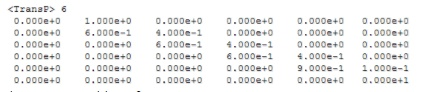
\includegraphics[width=0.5\textwidth]{states}
	\captionsetup{justification=centering}
	\caption{Transistions for 6 states}
\end{figure}

\subsubsection{HInnit}
HInnit builds an acoustic model for the name that has been passed in, using the trainList.txt it finds all the MFC vectors and looks through all the annotated .lab files to find the occurrences of the name. The acoustic model is trained using the parameters in the specified prototype file (test were carried out on different prototype files) which contains the vector size and the number of states. 
This whole process outputs the acoustic model for each trained name as a HMM in the HMM directory.

\subsubsection{HRest}
HRest re-trains the already made acoustic model from the HMM files. This can be ran as many times as wanted, we found that anymore than two times makes an insignificant difference to the correctness and accuracy of the results.
\subsubsection{HVite}
HVite is the first process of testing the acoustic model, it takes in all  MFC’s which are pointed to by the testList.txt. Compares the test MFC’s to the acoustic model and creates a results file containing the word utterances that are the closest match to the given data.


\subsubsection{HResults}
HResults is ran to give readable information on how well HVite ran on the test data. Given the label files for all the test data it takes in the result files from HVite, then  calculates the accuracy and correctness as well as outputting a confusion matrix.
Correctness = ((N - S - D)/N) x100     *
Accuracy = ((N - S - D - I)/N) x100    *
*N = number of items, H = hits (correctly recognized), S = Substitutions, D  = Deletions, I = Insertions. 

\subsubsection{Bash Script}
We developed a bash script to incorporate all these HTK features; from creating the model to testing it.
array:=[all names];
For each name in array
Do HInit;
Do HRest;
End loop
Do Hvite for test data;
Do HResults;

Each name of the 22 was placed into an array in which was iterated through and HInit was applied, outputting HMM files. For each HMM file the HRest was executed in the same loop. HVite is then used for the test data, then HResult creates the confusion matrix of the results

\section{Noise Compensation}
Background noise  was the most significant cause in the decrease of intelligibility of our speech recordings. The aim of our noise compensation techniques were to reduce the level of noise without affecting the quality of the speech too much. The noise compensation techniques we used are Spectral Subtraction and the Wiener Filter.

We initially added noise to our clean audio and then attempted to remove as much of that noise as possible in the hope of achieving a desirable signal-to-noise ratio (SNR). Once the noise was added to the audio, we saved the new audio to a file, then compared it to the original clean audio and the audio with the noise compensation techniques used. This way we could test for intelligibility and whether certain methods were giving us the best conceivable results. 

Once we had found what we had determined as the best technique for noise removal we then tested it against our acoustic model and altered the loudness of the noise and documented the accuracy decline with the increase in noise.

Our first step was to test our noise compensation techniques with some predefined noise, we then tested babble and our own lab noise

\subsection{Babble}
Speech babble is one of the most challenging noise interferences for all speech systems. Babble is incomprehensible speech usually consisting of multiple people in a room talking to each other with many different conversations happening asynchronously

We performed many tests with babble being added to the system. We originally began by adding babble to our training data and took measurements in the decline in accuracy when more babble was added to the testing data. 

We also tested our clean speech training data model against testing data with babble added and documented how to increase in db of the babble would decrease the accuracy of the results. See 6 for more information.
\subsection{Lab Noise}
When preparing for our demonstration we found that because the lab microphones had a reasonable amount of noise and the room itself contained a large amount of babble. This lead to poor results when recording testing data namely the system not recognising any points as silence.

In order to compensate for the poor quality of audio, In an attempt to replicate conditions in the laboratory we recorded a minute of silence in the computing labs to capture a representation of the sil periods on the annotated waveforms. This audio was then added to all training data at -20Db, see figure 11. 
\begin{figure}[ht]
	\centering
	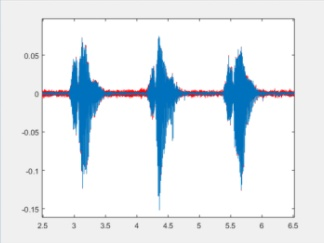
\includegraphics[width=0.4\textwidth]{noise}
	\captionsetup{justification=centering}
	\caption{Lab noise overlaid at -20db}
\end{figure}

After the development of the new training model the testing data was more accurately interpreted, meaning the silences were recognised and weren’t being replaced  with names.

\subsection{Spectral Subtraction}
The first noise compensation technique we used was Spectral subtraction. Spectral subtraction estimates an average of the speech spectrum and an average of  the noise spectrum in a given part of the audio and subtracts the noise from the speech, with the goal of improving the signal-to-noise ratio (SNR). 
\[x(n) = y(n) - d(n)\]

x(n) represents the new audio post spectral subtraction. 
The leading issue with spectral subtraction is that we don’t always know the noise signal d(n), which is why it is necessary to estimate the noise and subtract this from the noisy speech to given a further estimate of the clean speech.

In order to get this estimate we transferred to the frequency-domain as achieving time-domain noise estimate is difficult.
\[\hat{x}(n)=y(n)-\hat{d}(n)\]

We did this by taking the DFT of the time frame. And then subtracted the noise magnitude spectrum estimate. 
\[\left | \hat{X}(f) \right |=\left | Y(f) \right |- \left | \hat{D}(f) \right|\]

We then did the inverse DFT to initially review whether the speech is more intelligible.

\subsection{Wiener Filter}
Wiener filtering is one of the most widely used tools in signal processing and particularly for signal denoising and source separation. Wiener filter is typically applied in the time-frequency domain via the short-time Fourier transform (SFFT). \cite{DBLP:journals/spl/RouxV13}

The goal of the Wiener filter is to create an estimate of the clean signal from the corrupted by additive noise. It minimises the means square error between the estimated signal and the desired signal. \cite{DBLP:journals/ieiceee/Kim15}

\section{Evaluation}
During the development of the speech recognition system we executed various tests in order to achieve the best conceivable accuracy and system robustness. We did this by adding new training data (6.1), adding new test data (6.1.1), finding the optimal number of states (6.2), testing for optimal number of channels (6.3), finding the most efficient window (6.4), testing for optimal count of HRests (6.5), implementing MFCC (6.6), testing how noise affects the model (6.7), testing how babble affects the model (6.8), performing spectral subtraction (6.9) and the Wiener Filter (6.10).
\subsection{Additional Training Data}
 Once we had established a working model the first experiment we carried out was to trial our test data. We agreed the first step to improving the accuracy of the confusion matrix results would be to add more training data, this way it would allow for more variance in audio and hopefully pick up on more correct word utterances. Table 2 shows the process of adding extra training data to the model and the affect it had on the correctness and accuracy, the extra training is us recording each name again 10 and then 20 times.
 


\begin{table}[h]
	\caption{Adding extra training data}
	\centering
	\begin{tabular}{llr}
		
		\cmidrule(r){1-3}
		Extra Training & Correctness & Accuracy \\
		\midrule
		0 & 85.45 & 77.73 \\
		10  & 84.92  & 78.16 \\
		20   & 85.32  & 78.00 \\
		
	\end{tabular}
\end{table}
 As you can see from Table 2, the results are not as responsive as we had hoped. We concluded that the reasoning for the lack of noticeable increase in accuracy from the extra training data was that the conditions for the recordings were different.
 
  We essentially recorded the initial training data and test data on the same day at the same time in identical conditions, whereas the new additional data was recorded on a different day with potentially distinct conditions.
 
 \subsubsection{Adding test data}
 However, although the results for this test model were not as successful as originally hoped, with newly recorded test data the results were much more promising. 
 
 We recorded new testing data following the same format as before,
 this consisted of all 22 names spoken consecutively. More specifically , we recorded the new testing data in no explicit order; so the 22 names were scrambled and then spoken, we repeated this process 10 times.
 
 The correctness and accuracy of the new testing data against the original model ( With no added training data ) was 83.72 and 77.94 respectively. These results are less than the outcome of the original test data, which further suggests that the different conditions may be having an affect on the results. The correctness of the new testing data on the new training model was 85.83 and the accuracy was 83.12. This proves our hypothesis that the new training model allows for more variance in each speech utterance and has a more accurate representation of a speech recogniser.
 
 \textit{To ensure controlled experiments, the original training and testing data was used for the rest of the tests}
 
 


\subsection{Testing For Optimal Number Of States}
An HMM makes a transition from its current state to the one its connected to,
the probability of making a particular transition from state si to state sj is denoted by 
a transition probability. States are conditionally independent of all other states given the previous state and observations are conditionally independent of all other observations given the state that generated it. See \cite{DBLP:journals/ftsig/GalesY07} for more details.

We initially thought that the more states added to the speech recognition system, the more correct and accurate our results. We jumped to this conclusion because we originally tested for 4 states and then jumped straight to 20 with no in between.

We further then hypothesised that there is a chance the correctness and accuracy may plateau at a given number of states, so we decided to test incrementally by two states up to 18, see Table 3.
 
 \textit{For testing for the optimal number of states we used 20 channels.}

\begin{table}[h]
	\caption{Testing Different Number Of States}
	\centering
	\begin{tabular}{llr}
		
		\cmidrule(r){1-3}
		States & Correctness & Accuracy \\
		\midrule
		4 & 82.27 & -262 \\
		6  & 88.18  & 1.36 \\
		8   & 85.00  & 58.00 \\
	    10   & 85.45 & 77.73\\
	    12   & 86.82  & 84.55 \\
		14   & 87.27  & 85.40 \\
		16  & 87.27  & 85.45 \\
		18  & 87.27  & 85.45 \\
		
	\end{tabular}
\end{table}
The Table 3 results prove that our hypothesis was indeed correct, any higher than 14 states there was no increase in correctness and the Accuracy increase was minimal. This allowed us to make a conclusion that 14 is our optimal number of states.

States 4 and 6 had very poor accuracy because of a large number of insertion errors. More specifically the system wasn't picking up on the silences, rather than returning \textit{sil} it returned the word utterance in its place. This is the reasoning for the relatively high correctness as it was still picking up on the majority of the name utterances.

\subsection{Testing For Optimal Number Of Channels}
\textit{For testing for the optimal number of channels  we used our newly found optimal 14 states}.


For testing for the optimal number of channels we tested from 4 to 20 in increments of 2. We found that the higher the channel number the higher the correctness and accuracy. However we didn't increment further past 20 because we made the assumption that the increase in accuracy would be limited as the increase from 10-20 states was small. See Table 4 for more details.
\begin{table}[h]
	\caption{Testing Different Number Of Channels}
	\centering
	\begin{tabular}{llr}
		
		\cmidrule(r){1-3}
		Channels & Correctness & Accuracy \\
		\midrule
		4 & 55.91 & 37.73 \\
		6  & 70.91  & 62.27 \\
		8   & 76.36  & 70.91 \\
		10   & 84.09 & 78.64\\
		12   & 84.09  & 79.55 \\
		14   & 84.09  & 81.82 \\
		16  & 85.0  & 81.36 \\
		18  & 85.0  & 82.27 \\
		20  & 86.36  & 85.00 \\
	\end{tabular}
\end{table}

\subsection{Testing Different Windows}
In order to find the ideal speech recognition system we would have to find which window works best for our data. So we decided to test three of the main windows Hamming, Blackman-Harris and Hanning, see Table 5.

\textit{For comparing the different windows we used 14 states and 20 channels.}
\begin{table}[h]
	\caption{Changing the window}
	\centering
	\begin{tabular}{llr}
		
		\cmidrule(r){1-3}
		Window & Correctness & Accuracy \\
		\midrule
		Hamming & 86.36 & 85.00 \\
		Blackman-Harris  & 87.27  & 85.54 \\
		Hanning   & 86.36  & 85.45 \\
		
	\end{tabular}
\end{table}


We conclude that the window for the most correctness and accuracy is Blackman-Harris.


\textit{We continue to use Hamming window for the rest of the tests.}
\subsection{Using Multiple HRests}
HRest is used to refine the parameters of existing HMMs using Baum-Welch Re-estimation. We hypothesised that the more HRests commands executed, in theory, the more accurate our model should be. So we tested using multiple HRests and noticed it plateaued very quickly. This is shown in Table 6. 

\textit{We also tested with very large counts of HRests and noticed no change from having two} 
\begin{table}[h]
	\caption{Using Multiple HRests}
	\centering
	\begin{tabular}{llr}
		
		\cmidrule(r){1-3}
		Count & To & Name \\
		\midrule
		0 & 86.36 & 84.09 \\
        1  & 86.36  & 85.00 \\
		2  & 86.36  & 85.45 \\
	    4  & 86.36  & 85.45 \\
		
	\end{tabular}
\end{table}

\subsection{MFCC Results}
We implemented Mel-frequency cepstral coefficients using the same states, channels, training and testing audio to enable us to compare the results with Linear Frequency Cepstral Coefficients.

 Our results were not all that surprising as MFCC have been dominantly used in speech recognition globally. The correctness for MFCC was 96.55 and the accuracy was 95.24.

\subsection{Testing Noise On Clean Model}
We tested both MFCC and LFCC against a varying level of white noise from -30dB to 0dB.
After reading \cite{DBLP:conf/asru/ZhouGDES11} we hypothesised that MFCC would outperform in this test because the energy in high frequency region of speech is usually weak and it is more
susceptible to noise corruption. LFCC has more filterbanks in
the high frequency region and this is why it is less robust in
the white noise than MFCC. 

As you can see by Table 7 our results closely relate to our hypothesis 
\begin{table}[h]
	\caption{Testing Noise On Clean Model}
	\centering
	\begin{tabular}{llllr}
		
		\cmidrule(r){1-5}
		\centering  & LFCC & LFCC & MFCC & MFCC\\
		DB &  Correctness &  Accuracy &  Correctness  & Accuracy  \\
		\midrule
		-30 & 83.18 & 71.82 & 93.15 & 85.35 \\
		-20 & 58.62 & 29.51 & 72.75 & 45.12 \\
		-10 & 7.27 & 7.27 & 25.48 & 32.51 \\
		-0 & 4.55 & 4.55 & 10.42 & 14.52 \\
		
		
	\end{tabular}
\end{table}


\subsection{Testing Babble On Clean Model}
We tested both MFCC and LFCC against a varying level of Babble noise from -30dB to 0dB. Our original assumption was that because MFCC worked so efficiently when white noise was added that it would out perform LFCC in this scenario.

However, this was not the case as the results for LFCC were as good as and if not better than the results for MFCC, see Table 8.



\begin{table}[h]
	\caption{Testing Babble On Clean Model}
	\centering
	\begin{tabular}{llllr}
		
		\cmidrule(r){1-5}
		\centering  & LFCC & LFCC & MFCC & MFCC\\
		dB &  Correctness &  Accuracy &  Correctness  & Accuracy  \\
		\midrule
		-30 & 82.76 & 30.83 & 82.92 & 29.54 \\
		-20 & 75.45 & 11.36 & 76.21 & 10.24 \\
		-10 & 40.91 & 14.09 & 39.52 & 14.96 \\
		-0 & 8.45 & 8.45 & 8.30 & 8.35 \\
		
		
	\end{tabular}
\end{table}

The results show that LFCC is as robust as MFCC in
babble noise. These results compare to this paper \cite{DBLP:conf/asru/ZhouGDES11} , they concluded that LFCC should be more widely used for female trials by the mainstream of the speech-recognition community because it relates closely to speaker characteristics associated with the structure of the vocal tract, in particular the length of the vocal tract. Their results also concluded that LFCC is as robust as MFCC in babble noise.


\subsection{Performing Spectral Subtraction}
We added noise to our test data at different levels and performed spectral subtraction to the audio and then tested our results.

 For this given test we have the noise signal d(n), so we could easily spectrally subtract this from the noisy speech, however we wanted to replicate a real working noise compensation algorithm, so we transferred it to frequency-domain as it's much easier than retrieving the noise estimation in time-domain. We took the DFT of the time frame and then subtracted the noise magnitude spectrum estimate. Then inverse DFT to initially review whether the speech was intelligible

 \textit{We used LFCC for these tests}

\begin{table}[h]
	\caption{Performing Spectral Subtraction(With/Without spectral subtraction)}
	\begin{tabular}{llllr}
	
	\cmidrule(r){1-5}
	\centering  & Without & Without & With & With\\
	dB &  Correctness &  Accuracy &  Correctness  & Accuracy  \\
	\midrule
	-30 & 82.76 & 30.83 & 85.20 & 66.84\\
	-20 & 75.45 & 11.36 & 76.21 & 45.31 \\
	-10 & 40.91 & 14.09 & 50.73 & 39.41 \\
	-0 & 8.45 & 8.45 & 20.00 & 24.86 \\
	
	
\end{tabular}
\end{table}

Table 9 shows the improvement spectral subtraction has on both the Correctness and Accuracy of our results.



\subsection{Performing Wiener Filter}
We added noise to our test data at different levels and executed the Wiener filter on the audio and then tested our results.

From Table 10 it is clear that the Wiener filter increases the correctness and accuracy of the system, however it doesn't improve the results as effectively as Spectral Subtraction.

\begin{table}[h]
	\caption{Performing Wiener Filter(With/Without Filter subtraction)}
	\begin{tabular}{llllr}
		
		\cmidrule(r){1-5}
		\centering  & Without & Without & With & With\\
		dB &  Correctness &  Accuracy &  Correctness  & Accuracy  \\
		\midrule
		-30 & 82.76 & 30.83 & 83.16 & 42.63\\
		-20 & 75.45 & 11.36 & 75.45 & 29.93 \\
		-10 & 40.91 & 14.09 & 41.76 & 20.14 \\
		-0 & 8.45 & 8.45 & 15.22 & 14.52 \\
		
		
	\end{tabular}
\end{table}


\section{Conclusion}
From the tests executed we can devise a new optimal system, this includes an MFCC model with 14 states and 20 channels, 2 HRests and  Blackman-Harris window. This model is optimal provided the audio is clean. Also the model with the most amount of training data recorded in a variety of conditions will have the most success in terms of general speech-recognition.

If the audio is not clean and contains babble then we will alter the model to LFCC, also we will use spectral subtraction to remove the noise. However if the model contains white noise then we will keep it as is and use spectral subtraction to remove it.

The correctness and accuracy of the optimal model is 97.68 and 98.56 provided the audio is clean, these are our best results yet.




\clearpage
\bibliography{audiobibfile}{}
\bibliographystyle{plain}


\end{document}